\chapter{Thesis project: A standard MLOps CI/CD workflow}\label{ch:thesis-project:-a-standard-mlops-ci/cd-workflow}
\chaptermark{Thesis : MLOps WorkFlow}
\section{Introduction}\label{sec:introduction}
Following our state-of-the-art research we wanted to describe and implement a standard MLOps workflow.
I should be easily used on current project to improve their level of maturity or to initiate a new project with a solid
base to be fast in production.

We don't want to create a platform, but we want to use and integrate together reviewed
tools and workflows we encountered in the literature to propose our own.

\section{Tools}\label{sec:tools2}
In this section we will list all the tools we picked from our previous research.
As our workflow should be standard it should remain tools agnostic.

\subsection{Git Repositories and CI/CD}\label{subsec:github}
GitHub will be used to store and version control our codes repositories and configurations.
It will also be used to implement our CI/CD pipelines with GitHub actions.

\subsection{IAC, Containers and Registry}\label{subsec:dockerhub}
To benefit from containerization we will use docker to containerize our applications and models.
DockerHub will be used to store and version our Docker containers and Helm charts.

\subsection{Kubernetes}\label{subsec:kubernetes}
We will use a kubernetes cluster to benefit from its orchestration and deployment strategies.

\subsection{Airflow}\label{subsec:airflow}
We will use airflow for our DataOps pipelines and to integrate our kubeflow pipelines.


\subsection{Kubeflow}\label{subsec:kubeflow}
We will mainly use the storage solutions and pipelines offered by Kubeflow.
But by using kubeflow pipelines we could easily add features during the development.

\subsection{ArgoCD}\label{subsec:argocd}
ArgoCD will be used to implement our GitOps strategy and deploy our application, models, airflow and kubeflow.

\section{Infrastructure}\label{sec:infrastructure}

In figure\ref{fig:project-infra}, we describe our infrastructure that can be first deployed on a local kubernetes single node cluster
with independent DataOps and MLOps pipelines develop by different people with different roles.

by using airflow pipelines as general pipelines to trigger our kubeflow pipelines, we can easily gain in maturity towards
more automation by combining the DataOps pipelines and MLOps pipelines together when they are mature enough.

This way we enable kubeflow features for our model developers within a more general purpose environment.

By using the recent git/sync capabilities of Airflow we can synchronise our dags directly with airflow and
even trigger them automatically in a later stage towards automation.

We use Git Repositories for version control and triggering workflow pipeline runners.
We consider 4 types of repositories:

\begin{itemize}
    \item Code Repositories that holds code for models, libraries, docker images and infrastructure as code using Helm.
    \item MLOps and DataOps Pipelines Repositories.
    In our infrastructure those repositories holds the definition of our Airflow DAGs.
    In the first iteration those repositories can also hold images for
    \item Deployment/Configuration repositories.
    Those repositories are used to hold configuration for the deployed applications and Airflow dags.
    We use ArgoCD GitOps implementation to synchronise changes to those repositories.
    Airflow git/sync feature allows us to synchronise our dags with
    Change in those repositories can be automated by the pipeline runners.
    Depending on your team and organization those repositories can be separated into multiple repositories (per team, per domain, per environment (dev,test,staging,prod))
    For the Dev environment we allow developers to push from their code repositories within those repositories.
    For the production environment we use a pipeline to pull the configuration from the staging environment.
    We called this promote our configuration to a new environment.
    In case of full automation the pulling/promotion can be trigger automatically by ArgoCD sending webhooks on any test results desired.
    \item Workflow pipeline templates
    In those we define workflows that can be used in any repository to be used by the developers.
    It includes building image workflows, versioning with tags on repositories, pushing new configurations into deployments repositories.
    By defining them in a separate repository it allows us to version them and make it easy for developers to choose a workflow.
    Each workflow is closely tight to the structure of the repository, so we defined one per type of repositories.
\end{itemize}

\begin{figure}[!htbp]
    \centering
    \caption{Proposed MLOps kubernetes infrastructure using GitOps principles}
    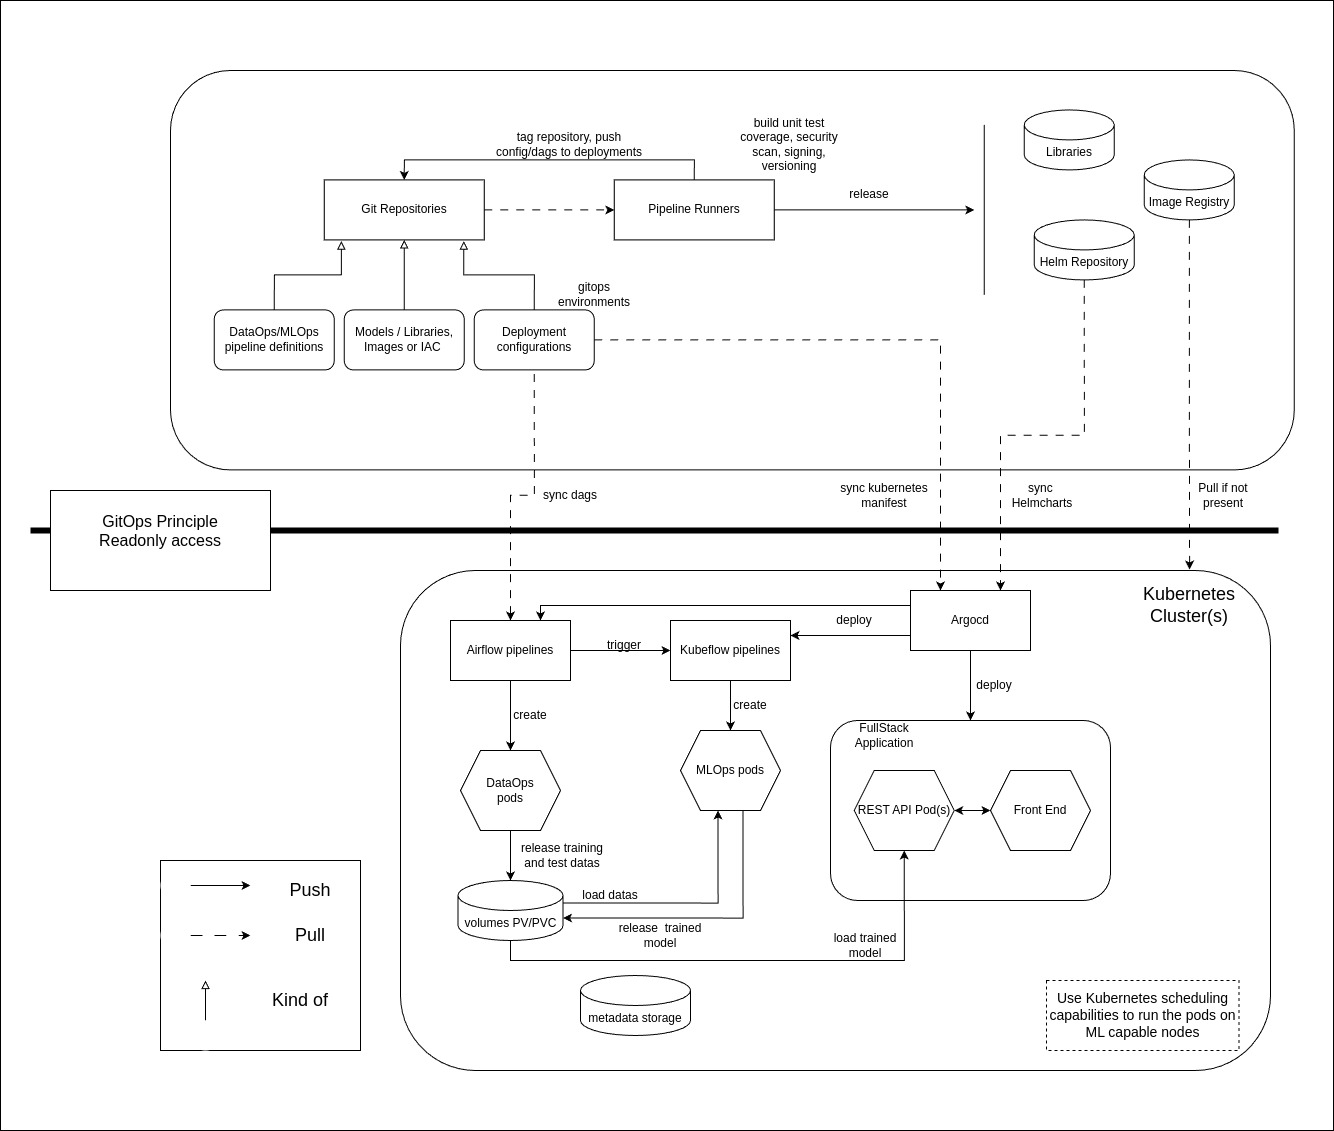
\includegraphics[scale=0.35]{images/project/mthmlops-infra}
    \label{fig:project-infra}
\end{figure}


\section{Workflow}\label{sec:workflow}
As we explained while describing the infrastructure, part of our global workflow can be implemented within pipelines runners definition.
We used GitHub action and the GitHub flow to harmonise the workflow within our different type of git repositories.
GitHub allows us to define template in a single repository that can be then versioned and used in other repositories while hiding the complexity of the defined pipelines.



\section{Conclusion}\label{sec:conclusion}
Airflow pipelines and kubeflow pipelines to easily integrate DataOps and MLOps pipelines together to reach more automation as the project gains maturity.
